% !TeX spellcheck = pl_PL
\documentclass[10pt, a4paper]{article}
\usepackage[lmargin=40mm, rmargin=40mm, tmargin=52mm, bmargin=52mm, foot=0mm, head=0mm]{geometry}
\setlength{\parindent}{10mm}

% Lista wszystkich języków stanowiących języki pozycji bibliograficznych użytych w pracy.
% (Zgodnie z zasadami tworzenia bibliografii każda pozycja powinna zostać utworzona zgodnie z zasadami języka, w którym dana publikacja została napisana.)
\usepackage[english,polish]{babel}

% Użyj polskiego łamania wyrazów (zamiast domyślnego angielskiego).
\usepackage{polski}

\usepackage[utf8]{inputenc}

% dodatkowe pakiety
\usepackage{mathtools}
\usepackage{amsfonts}
\usepackage{amsmath}
\usepackage{amsthm}
\usepackage{bm}
\usepackage{adjustbox}
\usepackage[dvipsnames]{xcolor}
\usepackage{pgfplots}
\let\pgfimage\includegraphics % pgfimage doesn't work with \import
% \usepackage{textcomp}

% obrazki
\usepackage{graphicx}
\usepackage{rotating}
\usepackage[font=small, labelfont=bf, labelsep=period]{caption}
\usepackage{subcaption}
\usepackage{float}
\captionsetup{justification=centering}

% --- < bibliografia > ---

\usepackage{placeins}	% poprawia float

\let\Oldsection\section
\renewcommand{\section}{\FloatBarrier\Oldsection}

\let\Oldsubsection\subsection
\renewcommand{\subsection}{\FloatBarrier\Oldsubsection}

\let\Oldsubsubsection\subsubsection
\renewcommand{\subsubsection}{\FloatBarrier\Oldsubsubsection}

\usepackage[explicit]{titlesec}
\titleformat{\section}[block]
{\large\centering}{\thesection. \MakeUppercase{#1}}{0ex}{}
\titlespacing{\section}{0pt}{11pt plus 0pt minus 1pt}{11pt plus 0pt minus 1pt}
\titleformat{\subsection}[block]
{\normalsize\centering}{\thesubsection. \MakeUppercase{#1}}{0ex}{}
% \titlespacing{\subsection}{8pt}{8pt}{2.5mm}


\usepackage[
style=numeric,
sorting=none,
% Zastosuj styl wpisu bibliograficznego właściwy językowi publikacji.
language=autobib,
autolang=other,
% Zapisuj datę dostępu do strony WWW w formacie RRRR-MM-DD
%urldate=iso,
%seconds=true,
% Nie dodawaj numerów stron, na których występuje cytowanie
backref=false,
% Podawaj ISBN.
isbn=true,
% Nie podawaj URL-i, o ile nie jest to konieczne
url=false,
% Ustawienia związane z polskimi normami dla bibliografii
maxbibnames=6,
minbibnames=6,
% Jeżeli używamy Bibera:
backend=biber
]{biblatex}

\renewcommand\UrlFont{\rmfamily\itshape}

\AtBeginBibliography{
  \renewcommand\labelnamepunct{,\space}
  \renewcommand\newunitpunct{\addcomma\space}
  \renewcommand{\finentrypunct}{}

  \renewcommand{\bibopenparen}{\addcomma\addspace}
  \renewcommand{\bibcloseparen}{\addspace}
}

\usepackage{csquotes}
% Ponieważ `csquotes` nie posiada polskiego stylu, można skorzystać z mocno zbliżonego stylu chorwackiego.
\DeclareQuoteAlias{croatian}{polish}


\usepackage{indentfirst}
% Przecinki do numerów
\usepackage{icomma}
% ------------------------
%---------------------------------------------------------------------------
% Ustawienia wyświetlania liczb (zgodne z polskimi zwyczajami typograficznymi)
%---------------------------------------------------------------------------
\usepackage[detect-weight=true, detect-family=true]{siunitx}
\sisetup{
  output-decimal-marker = {,},
  %	round-mode=places,
  %	round-precision=4,
  group-separator={~},
}

% --- < listingi > ---

% Użyj czcionki kroju Times.
\usepackage{newtxtext}
\usepackage{anyfontsize}
\usepackage[all,defaultlines=2]{nowidow}

\usepackage{listings}
\lstloadlanguages{TeX}

\lstset{
  literate={ą}{{\k{a}}}1
  {ć}{{\'c}}1
  {ę}{{\k{e}}}1
  {ó}{{\'o}}1
  {ń}{{\'n}}1
  {ł}{{\l{}}}1
  {ś}{{\'s}}1
  {ź}{{\'z}}1
  {ż}{{\.z}}1
  {Ą}{{\k{A}}}1
  {Ć}{{\'C}}1
  {Ę}{{\k{E}}}1
  {Ó}{{\'O}}1
  {Ń}{{\'N}}1
  {Ł}{{\L{}}}1
  {Ś}{{\'S}}1
  {Ź}{{\'Z}}1
  {Ż}{{\.Z}}1,
  basicstyle=\footnotesize\ttfamily,
}

% ------------------------

\AtBeginDocument{
  \renewcommand{\tablename}{\textbf{Tabela}}
  \renewcommand{\figurename}{\textbf{Rysunek}}
}

% ------------------------
% --- < tabele > ---

\usepackage{array}
\usepackage{tabularx}
\usepackage{multirow}
\usepackage{booktabs}
\usepackage{makecell}
\usepackage[flushleft]{threeparttable}

% defines the X column to use m (\parbox[c]) instead of p (`parbox[t]`)
\newcolumntype{C}[1]{>{\hsize=#1\hsize\centering\arraybackslash}X}

% \setlength{\cftsecnumwidth}{10mm}
% \setcounter{secnumdepth}{4}
% \brokenpenalty=10000\relax

% ------------------------
% --- < do tego artykułu > ---
\sisetup{binary-units=true}
\DeclareSIUnit{\inch}{"}
\usepackage{import}

%---------------------------------------------------------
% Nazwa pliku z bibliografią
%---------------------------------------------------------
\addbibresource{bibliografia.bib}

\begin{document}

\pagestyle{empty}

\begin{center}
  \large\textbf{\MakeUppercase{Wielokanałowy system syntezy pola akustycznego oparty o mikrokomputery Raspberry Pi}}
\end{center}
\vspace{22pt}

\noindent\MakeUppercase{M. Piszak} (uczestnik Konkursu Prac Studenckich), \MakeUppercase{S.~Mikulicz, M.~Kmiecik,} \linebreak \MakeUppercase{T.~Makuch, P.~Pawlik} (opiekun naukowy)\\

\noindent AGH Akademia Górniczo-Hutnicza im. S. Staszica w Krakowie, Wydział Inżynierii Mechanicznej i~Robotyki, Katedra Mechaniki i~Wibroakustyki
\\

\noindent piszak@student.agh.edu.pl

\vspace{22pt}

W większości systemów reprodukcji dźwięku wrażenia słuchowe są zależne od pozycji słuchacza. Technologią pozwalającą na usunięcie tego ograniczenia jest Wave Field Synthesis (WFS, Synteza Pola Akustycznego). Dzięki odpowiedniemu przetwarzaniu sygnałów, macierz głośników pozwala na formowanie kształtu czoła fali akustycznej tak, aby symulować wirtualne źródło dźwięku w~dowolnej odległości od słuchacza, niezależnie od jego pozycji.

Wykorzystujące tę metodę systemy są zazwyczaj skomplikowane i~drogie ze względu na wymaganą dużą liczbę niezależnych kanałów przetwarzania DSP i~przetworników elektroakustycznych. Projekt obejmuje stworzenie modułowego systemu WFS opartego na mikrokomputerach Raspberry Pi (RPi) oraz dedykowanych modułach wzmacniaczy klasy D~wyposażonych w~przetworniki cyfrowo-analogowe. Modułowość konstrukcji pozwala na jednoczesne niezależne przetwarzanie dużej liczby sygnałów oraz skonfigurowanie systemu w~dowolny sposób, a~także umożliwia rozszerzanie systemu o~kolejne zestawy głośników, co zwiększa dokładność syntezy.

Obok właściwego przetwarzania sygnałów w~zależności od lokalizacji źródła, głównym wyzwaniem była synchronizacja odtwarzania przez wiele niezależnych modułów RPi -- precyzja synchronizacji jest kluczowa dla jakości generowania pola akustycznego oraz percepcji zgodnej z~założeniami. Dlatego wprowadzono rozwiązanie pozwalające na synchronizację odtwarzania dźwięku przez wszystkie moduły.

Skonstruowano działający prototyp systemu, którego działanie zostało poddane weryfikacji pomiarowej. Wykonano pomiary sygnału na wyjściu każdego wzmacniacza oraz wstępne pomiary w~komorze bezechowej, pozwalające określić jakość pola akustycznego generowanego przez skonstruowany system.

\section{Wprowadzenie}

Wspólną cechą większości systemów reprodukcji dźwięku przestrzennego jest 
ograniczenie odsłuchu do niewielkiego obszaru (tzw. \textit{sweet spot}).
Metodą pozwalającą na oddanie wrażeń przestrzennych także gdy słuchacz jest 
w~ruchu lub dla kilku słuchaczy jednocześnie, bez konieczności używania przez
nich słuchawek, jest synteza pola akustycznego, ang. \textit{Wave Field Synthesis}
(WFS).

Celem niniejszej pracy było zaprojektowanie oraz skonstruowanie modułowego systemu
syntezy pola akustycznego, składającego się z~łatwo dostępnych komponentów
\linebreak i~umożliwiającego stosunkowo prostą adaptację do wybranego zastosowania.

Metoda WFS oparta jest na zasadzie Huygensa: każdy punkt do którego dociera
fala akustyczna staje się źródłem nowej fali. Zgodnie z tą zasadą każdy głośnik
w~macierzy może być rozpatrywany zarówno jako odbiornik (punkt, do którego
dociera fala dźwiękowa) jak i~jako źródło drugiego rzędu, reprodukujące falę
pochodzącą od źródła wirtualnego (rys.~\ref{r:Huygens}). Dzięki
odpowiedniemu przetwarzaniu sygnału głośniki emitują fale, które nakładając
się tworzą wrażenie źródła zlokalizowanego w~określonym punkcie w~przestrzeni~\cite{hq_rendering} (rys.\ref{r:symulacja}).

\begin{figure}[!tbh]
  \centering
  \begin{subfigure}[b]{.49\textwidth}
    \centering
    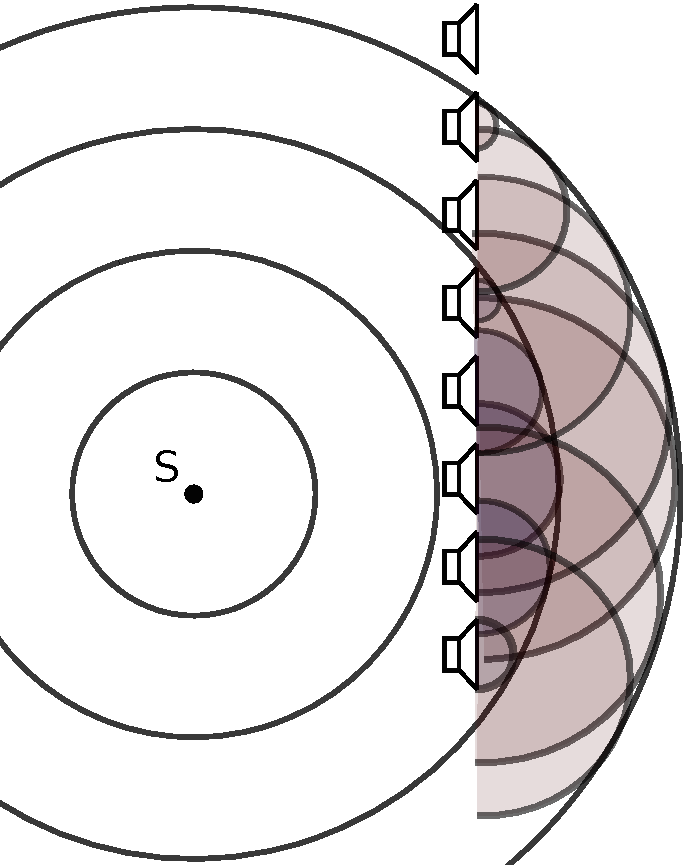
\includegraphics[scale=.35]{vecgraphics/WFS_idea.pdf}
    \caption{Zastosowanie zasady Huygensa w WFS: każdy głośnik jest punktem do
    którego dociera fala wyemitowana przez wirtualne źródło}
    \label{r:Huygens}
  \end{subfigure}
  ~
  \begin{subfigure}[b]{.49\textwidth}
    \centering
    \adjustbox{max width=\textwidth}{\import{./vecgraphics/}{symulacja200Hz.pdf_tex}}
    \caption{Wyznaczony analitycznie rozkład pola generowanego przez zaprojektowany system dla fali sinusoidalnej o~częstotliwości \SI{200}{\hertz}}
    \label{r:symulacja}
  \end{subfigure}
  \caption{Ilustracja zasady działania systemu WFS}
\end{figure}

Równaniem, na którym opiera się przetwarzanie sygnałów w~WFS jest całka
Helmholtza-Huygensa,
pozwalająca wyznaczyć analitycznie rozkład ciśnienia akustycznego pochodzącego od danego
zestawu źródeł~\cite{snaka}. Na tej podstawie definiowana jest funkcja
opisująca ciśnienie akustyczne w~punkcie umieszczenia każdego głośnika (zob. rozdział~\ref{s:algorithm}). To
podejście pozwala uwzględnić geometrię przestrzeni i~straty energii podczas
propagacji fali dźwiękowej oraz wyznaczyć amplitudy i~fazy sygnału dla każdego
z~głośników. 

\section{Projekt systemu}

W ramach projektowania systemu między innymi: (1) wybrano rozmiar macierzy
głośnikowej i~dobrano odpowiednie przetworniki oraz dobrano pozostałe elementy
systemu; (2) zaprojektowano algorytm przetwarzania sygnałów; (3) przeprowadzono
symulacje rozkładu pola akustycznego, by zweryfikować działanie algorytmu.

\subsection{Geometria}

Rozmiar macierzy głośnikowej determinuje zakres częstotliwości, w~którym system
jest w~stanie odtwarzać dźwięk z dużą dokładnością. Przyjęte w modelu teoretycznym 
źródło liniowe jest w~rzeczywistości szeregiem dyskretnych źródeł, oddalonych od siebie 
o~odległość $\Delta x$, a~każdy głośnik ma określone wymiary. Im większa macierz, tym niższa
jest minimalna częstotliwość, która może być poprawnie odtworzona $f_{min}$ --- źródło jest wystarczająco duże w stosunku 
do długości fali akustycznej ($f_{min}>\frac{c}{L}$, gdzie $c$~oznacza prędkość propagacji fali dźwiękowej,
a~$L$~to długość macierzy głośników).

Dla górnej granicy częstotliwości należy uwzględnić zjawisko aliasingu
przestrzennego. Odległości pomiędzy głośnikami powodują różnice fazowe, w~wyniku których 
występuje konstruktywna i~destruktywna interferencja dla częstotliwości powyżej~\eqref{eq:fmax}:

\begin{equation}
  f_{max}=\frac{c}{2\Delta x \sin{\alpha_{max}}} \quad, \label{eq:fmax}
\end{equation}
gdzie:\\
\indent \begin{tabular}{l c p{.69\textwidth}}
  $f_{max}$ [\si{\hertz}] & --- & najwyższa częstotliwość wolna od aliasingu przestrzennego, \\
  $\Delta x$ [\si{\metre}] & --- & odległość między środkami dwóch sąsiednich głośników, \\
  $\alpha_{max}$ [\si{\radian}] & --- & maksymalny kąt pomiędzy falą padającą od źródła 
  wirtualnego a~płaszczyzną przebiegającą przez membrany wszystkich głośników w~macierzy.\\
\end{tabular}\\

Efekt ten nie zniekształca jednak dźwięku w sposób znaczący dla odbioru przez 
słuchacza~\cite{hq_rendering}.

Uwzględniając te ograniczenia, zdecydowano się wykorzystać głośniki o średnicy \SI{3}{\inch}
(\SI{81}{\milli\meter}), które rozmieszczono co $\Delta x=\SI{150}{\milli\meter}$.

\subsection{Przetwarzanie sygnałów}\label{s:algorithm}

Dla określonej geometrii układu źródło wirtualne --- macierz głośników,
korzystając z~całki Helmholtza-Huygensa, widmo sygnału podawanego na każdy głośnik można zapisać
w~postaci~\eqref{eq:glosnik_f}~\cite{enhancement}:

\begin{equation}
  Q_n(\bm{r}_n,\omega) = \sqrt{\frac{jk}{2\pi}} A_n \frac {e^{-jk|\bm{r}_n-\bm{r}_m|}}{|\bm{r}_n-\bm{r}_m|^{1/2}} S(\omega) \quad,
  \label{eq:glosnik_f}
\end{equation}
gdzie:\\
\indent \begin{tabular}{l c p{.7\textwidth}}
  $\bm{r}_n$ & --- & wektor opisujący położenie głośnika, \\
  $\bm{r}_m$ & --- & wektor opisujący położenie źródła wirtualnego,\\
  $A_n$ & --- & współczynnik wagowy amplitudy,\\
  $k$ & --- & liczba falowa,\\
  $S(\omega)$ & --- & widmo sygnału źródłowego.
\end{tabular}\\

Zastosowano przetwarzanie w~dziedzinie częstotliwości, ponieważ na tym etapie jest ono bardziej efektywne
--- zamiast wykonywania kosztownej obliczeniowo operacji splotu, widmo sygnału przemnażane jest przez
odpowiednie współczynniki.

\section{Realizacja}

Zastosowano rozwiązania oparte na mikrokomputerach Raspberry
Pi. Mają one niewielkie wymiary i~dysponują odpowiednią mocą obliczeniową
potrzebną do przetwarzania sygnałów wysyłanych na poszczególne kanały.

Przetwarzanie sygnału z~cyfrowego na analogowy oraz jego wzmocnienie jest
realizowane przez moduł Amp Zero pHAT firmy JustBoom. Jest to połączenie
przetwornika analogowo-cyfrowego oraz wzmacniacza klasy D~o~mocy wyjściowej
$2\times40\si{\watt}$. Sygnał może być próbkowany z~częstotliwością
\SI{192}{\kilo\hertz} i~rozdzielczością \num{32} bitów, a~zastosowanie
wzmacniacza klasy D~umożliwia osiąganie odpowiedniej mocy głośników przy
zachowaniu niewielkich rozmiarów pojedynczego modułu.

Jako przetworników elektroakustycznych użyto głośników firmy Faital Pro, model 3FE25,
o~średnicy \SI{3}{\inch}, impedancji \SI{8}{\ohm} i~nominalnym zakresie 
częstotliwości \SI{100}{\hertz}~--~\SI{20}{\kilo\hertz}.

Każdy moduł składa się z~komputera Raspberry Pi, modułu wzmacniacza Amp Zero
oraz dwóch głośników. 
Strukturę systemu przedstawia rysunek \ref{fig:schemat}.

\begin{figure}[!tbh]
  \centering
  \adjustbox{max width=.7\linewidth}{\import{./vecgraphics/}{scheme3.pdf_tex}}
  \caption{Schemat projektowanego systemu WFS}
  \label{fig:schemat}
\end{figure}

Aby generowane pole akustyczne było spójne, nie mogą wystąpić dewiacje czasu
przetwarzania sygnałów przez poszczególne moduły. Dlatego system posiada połączenie
synchronizujące moment rozpoczęcia odtwarzania próbek dźwięku.

Połączenie synchronizujące wykorzystuje piny GPIO (piny ogólnego przeznaczenia, ang.
\textit{General Purpose Input-Output}), oprogramowanie napisano w~języku 
Rust, korzystając z~biblioteki 
\emph{RPPAL}~\cite{RPPAL}. Dane audio oraz informacje na temat wzajemnego położenia 
głośników i~wirtualnego źródła przesyłane są bezprzewodowo przez sieć lokalną, co
oznacza, że system nie odtwarza dźwięku w~czasie rzeczywistym, ale
pozwala na wygodne modyfikacje układu przestrzennego i~zmniejsza ilość
przewodów. Główna jednostka systemu z~aplikacją serwera kontroluje połączenie
synchronizujące oraz zarządza procesami przetwarzania audio.

\section{Pomiary weryfikujące}

W~celu weryfikacji działania systemu synchronizacji oraz ewentualnego wykrycia innych 
problemów zmierzono sygnały na wyjściu wszystkich wzmacniaczy. [\textit{opis pomiarów + wyniki}]

Wykonano także wstępne pomiary rozkładu pola akustycznego generowanego przez system 
w~komorze bezechowej: zarejestrowano przebieg ciśnienia akustycznego w~32 punktach 
rozmieszczonych co~\SI{400}{\milli\metre}, dla różnych pozycji źródła wirtualnego. 
Na rysunku~\ref{r:pomiar_kb}, przedstawiającym wyniki pomiaru dla tej samej pozycji 
źródła, dla której wykonano obliczenia analityczne, można zauważyć,
że kształt czoła fali jest zbliżony do oczekiwanego (zob. rys.~\ref{r:symulacja}).

\begin{figure}[!tbh]
  \centering
  \begin{subfigure}[b]{.49\textwidth}
    \centering
    % 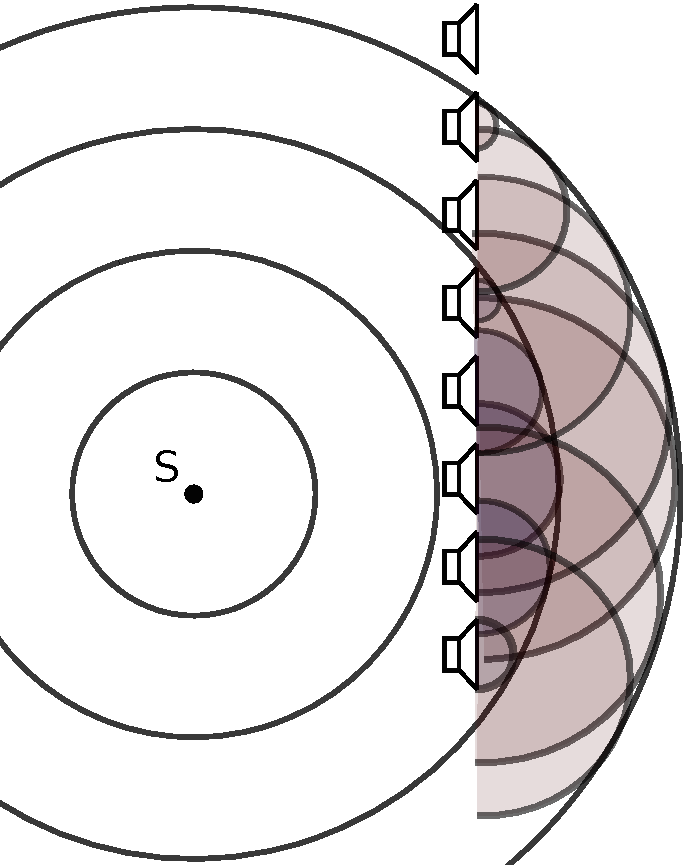
\includegraphics[scale=.35]{vecgraphics/WFS_idea.pdf}
    \caption{Wyniki pomiaru sygnału na wyjściu wzmacniaczy}
    \label{r:pomiar_el}
  \end{subfigure}
  ~
  \begin{subfigure}[b]{.49\textwidth}
    \centering
    \import{./plots/}{sin200_s5_IAB.pgf}
    \caption{Interpolowany rozkład pola dla fali sinusoidalnej o~częstotliwości \SI{200}{\hertz}}
    \label{r:pomiar_kb}
  \end{subfigure}
  \caption{Wyniki pomiarów prototypu}
\end{figure}

\section{Podsumowanie}

Skonstruowano działający system WFS spełniający podstawowe założenia tej metody.
W~ramach dalszych prac system zostanie rozbudowany o~kolejne funkcjonalności,
takie jak m.in. obudowy głośników, interfejs użytkownika umożliwiający sterowanie 
parametrami źródeł wirtualnych, synteza dźwięku dla ruchomych źródeł.

Dzięki swojej modułowości, zaprojektowany system może zostać dostosowany do 
konkretnego zastosowania poprzez odpowiednie ustawienie głośników. Ponadto,
jego skonstruowanie wiąże się ze znacznie mniejszymi kosztami, niż typowego
systemu WFS.

Zastosowania syntezy pola akustycznego obejmują przemysł rozrywkowy, poprawę
jakości akustyki pomieszczeń~\cite{enhancement}, badania psychoakustyczne,
oraz dydaktykę -- zaprojektowany system można dostosować do każdego z~nich.
Ponadto może być on użyty do dalszych badań nad możliwościami i ograniczeniami
tej metody reprodukcji dźwięku.

\printbibliography

\end{document}
